% Chapter 6 — GPU Architecture, CUDA Programming, and Maximizing Occupancy  (v2: narrative edition)
% 53 pages; Part I follows the BOOK section order (SM internals -> threads/warps/blocks/grids -> limits -> PTX);
% 4 presenter intuition pages at 7, 9, 14, 15. Page numbers differ from v1. Use chapter06-lecture-script-v2-zh.md.
% v2 changes: book-plan opening (p2: SIMT -> CUDA -> memory -> roofline), question-driven roadmap (p3), worked-example p14, takeaway titles,
% unified workshop metaphor, occupancy caveat at p16, part-transition bridges, Plain-English takeaway bars.
% Compile: pdflatex chapter06-presentation-v2.tex  (run twice)
\documentclass[aspectratio=169]{beamer}

% ====== Presenter info: EDIT ME ======
\newcommand{\PresenterName}{Tianqin Cai}          % <-- 改成你的名字
\newcommand{\PresenterTitle}{Applied Scientist} % <-- 改成你的头衔
\newcommand{\PresenterOrg}{AWS}
% =====================================

\usetheme{Madrid}
\definecolor{navy}{RGB}{18,47,90}
\definecolor{kwblue}{RGB}{0,56,132}
\definecolor{okgreen}{RGB}{80,130,20}
\usecolortheme[named=navy]{structure}
\setbeamercolor{frametitle}{bg=navy,fg=white}
\setbeamercolor{title}{bg=navy,fg=white}
\setbeamercolor{block title}{bg=navy,fg=white}
\setbeamercolor{block body}{bg=gray!12,fg=black}
\setbeamercolor{block title example}{bg=okgreen,fg=white}
\setbeamercolor{block body example}{bg=okgreen!10,fg=black}
\setbeamertemplate{navigation symbols}{}
\setbeamertemplate{blocks}[rounded][shadow=true]

\usepackage{booktabs}
\usepackage{listings}
\lstset{
  language=C++,
  basicstyle=\ttfamily\fontsize{6.5}{7.6}\selectfont,
  keywordstyle=\color{kwblue}\bfseries,
  commentstyle=\color{gray}\itshape,
  stringstyle=\color{okgreen},
  showstringspaces=false,
  breaklines=true,
  columns=fullflexible
}

\newcommand{\kw}[1]{\textbf{\textcolor{kwblue}{#1}}}
\newcommand{\pe}[1]{\par{\setlength{\fboxsep}{2.5pt}\noindent\colorbox{navy!9}{\parbox{\dimexpr\textwidth-5pt\relax}{\footnotesize\itshape Plain English: #1}}}}
\newcommand{\bridge}[1]{{\footnotesize\itshape\textcolor{gray}{#1}}\par}
\newcommand{\refmark}[1]{\textsuperscript{[#1]}}

\title[AI Systems Performance Engineering]{AI Systems Performance Engineering}
\subtitle{Chapter 6 --- GPU Architecture, CUDA Programming, and Maximizing Occupancy\\{\small Part I structure preview (draft)}}
\author[\PresenterName\ \ \PresenterTitle\ \ \PresenterOrg]{\PresenterName\\\PresenterTitle\\\PresenterOrg}
\institute[]{\footnotesize Internal Training for Applied Scientists on AI Infrastructure}
\date{August 15, 2026}

\begin{document}

% ================================================================ 1
\begin{frame}
  \titlepage
\end{frame}

% ================================================================ 2
\begin{frame}{What This Chapter Covers}
  \begin{enumerate}
    \item \kw{SIMT execution model} --- how \kw{warps}, \kw{thread blocks}, and \kw{grids}
          map your algorithm onto \kw{SMs}. \hfill (Part I)
    \item \kw{CUDA programming patterns} --- kernel anatomy, launch parameters,
          asynchronous allocation. \hfill (Part II)
    \item \kw{Memory hierarchy} --- register file, shared/L1, L2, HBM3e, plus
          asynchronous data movement (\kw{TMA}, \kw{TMEM}). \hfill (Part III)
    \item \kw{Roofline analysis} --- is a kernel \kw{compute-bound} or \kw{memory-bound}?
          Push toward \kw{peak throughput}. \hfill (Parts IV--V)
  \end{enumerate}
  \medskip
  \begin{block}{Where does occupancy fit?}
    \small Occupancy is the working metric that connects the SIMT model (Part I) to peak
    throughput (Parts IV--V): enough \kw{resident warps} keep SMs busy while data moves.
  \end{block}
  \pe{the arc: \kw{how the GPU executes} $\to$ how you program it $\to$ where data lives $\to$ \kw{what limits speed}.}
\end{frame}

% ================================================================ 3
\begin{frame}{Roadmap: Five Parts, Each Answers One Question}
  \begingroup\small\setlength{\tabcolsep}{6pt}\renewcommand{\arraystretch}{1.25}
  \begin{tabular}{@{}lll@{}}
    \toprule
    \textbf{Part} & \textbf{Slides} & \textbf{The question it answers} \\
    \midrule
    I \ GPU architecture & 4--20 & How does \kw{SIMT} map warps/blocks/grids onto SMs? \\
    II \ CUDA programming & 21--28 & How do we \kw{map a computation onto GPU threads}? \\
    III \ Memory hierarchy & 29--37 & Where does data \kw{live}, and what does \kw{movement cost}? \\
    IV \ Occupancy in practice & 38--46 & \kw{When} do more warps actually help? \\
    V \ Correctness \& roofline & 47--50 & Optimize \kw{compute} next, or \kw{memory}? \\
    \bottomrule
  \end{tabular}\endgroup
  \bigskip
  \begin{block}{The whole chapter in one sentence}
    \centering \kw{Expose enough parallelism, keep data close, and profile the real bottleneck.}
  \end{block}
  \medskip
  \centering\footnotesize\itshape
  When a detail page appears (SFU, TMEM, Unified Memory\ldots), it always belongs to one of these five questions.
\end{frame}

% ================================================================ 4
\begin{frame}{Part I --- GPUs Optimize Throughput; CPUs Optimize Latency}
  \begin{columns}[c]
    \column{0.55\textwidth}
    \begin{itemize}
      \item CPUs: few cores, deep caches, fast \emph{single} threads. GPUs: hundreds of \kw{SMs}
            (streaming multiprocessors) running \kw{thousands of threads} in parallel.
      \item Basic CUDA flow (right): host copies data \kw{CPU $\to$ GPU}, launches a \kw{kernel},
            copies results back.
      \item The GPU's edge is \kw{massive parallelism}: many SMs process different data
            \kw{at once}; within an SM, \kw{resident warps} also fill memory stalls.
      \item Sweet spot: \kw{data-parallel} work --- matrix multiplies, convolutions ---
            written in CUDA C++ or via \kw{PyTorch} / OpenAI \kw{Triton}.\refmark{1,3}
    \end{itemize}
    \column{0.42\textwidth}
    \centering
    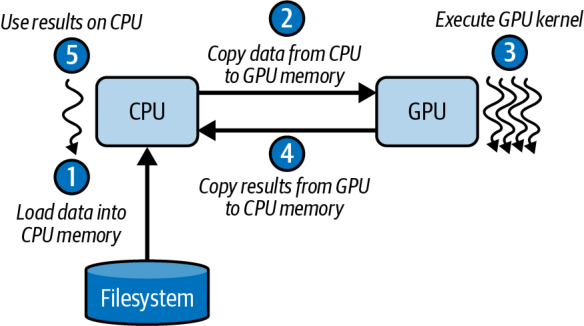
\includegraphics[width=0.88\linewidth]{figs/fig6-1.png}\\
    {\scriptsize Figure 6-1. Simple CUDA programming flow}
  \end{columns}
  \pe{the CPU finishes one part fast; the GPU is a \kw{factory} --- keep \kw{every workshop busy}.}
\end{frame}

% ================================================================ 5
\begin{frame}{Inside a Blackwell SM: The Resource Budget}
  \begin{columns}[c]
    \column{0.52\textwidth}
    \begin{itemize}
      \item Each SM tracks up to \kw{64 warps} (\kw{warp} = 32 threads; details p.~13)
            = \kw{2{,}048 threads} --- the pool the scheduler switches between.
      \item \kw{64K 32-bit registers} per SM (256 KB total); any single thread can use
            at most \kw{255}.
      \item \kw{256 KB} combined L1 cache / shared memory; up to \kw{228 KB} configurable as
            user-managed shared memory (\kw{227 KB usable} --- CUDA reserves 1 KB per block).
      \item These on-chip budgets let one SM juggle thousands of threads without
            constantly touching DRAM.\refmark{2}
    \end{itemize}
    \column{0.45\textwidth}
    \centering
    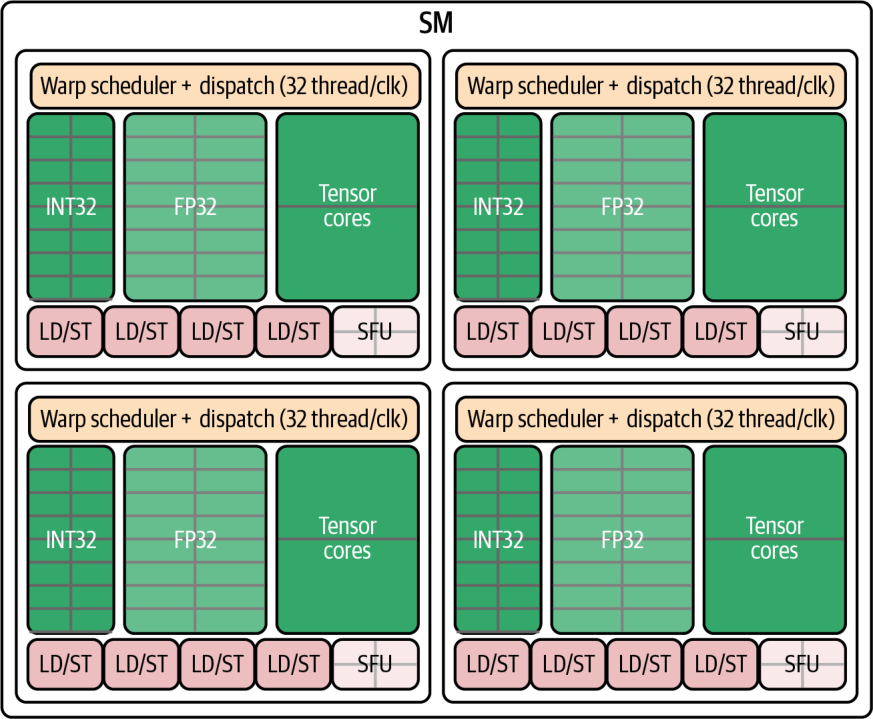
\includegraphics[width=0.8\linewidth]{figs/fig6-2.png}\\
    {\scriptsize Figure 6-2. A Blackwell SM: four scheduling partitions sharing on-chip resources}
  \end{columns}
  \pe{an SM is a workshop: registers are toolbelts, shared memory is the workbench.}
\end{frame}

% ================================================================ 6
\begin{frame}{SFUs and Load/Store Pipelines}
  \begin{columns}[t]
    \column{0.48\textwidth}
    \begin{block}{SFU --- Special Function Unit}
      \begin{itemize}\small
        \item Handles \kw{transcendentals}: sine, cosine, reciprocal, square root.
        \item Own \kw{dedicated pipeline} --- \emph{not} part of the dual-issue math+memory pair (p.~8).
        \item Slow functions never stall the core compute/memory pipes $\Rightarrow$
              more \kw{instruction-level parallelism} for mixed-operation kernels.
      \end{itemize}
    \end{block}
    \column{0.48\textwidth}
    \begin{block}{LD/ST --- Load/Store pipelines}
      \begin{itemize}\small
        \item \kw{16 LD/ST pipelines} per SM (4 per scheduler) feed L1/shared, L2, and global memory.
        \item \kw{Caveat (book warning):} exact counts and pairings are \kw{not guaranteed} ---
              rely on profiling counters and the \kw{Blackwell tuning guide}.\refmark{2}
      \end{itemize}
    \end{block}
  \end{columns}
  \pe{the SFU is a specialist counter at the back of the store --- complicated requests go there so the express lanes keep moving.}
\end{frame}

% ================================================================ 7
\begin{frame}{Analogy: The GPU as a Factory}
  \centering
  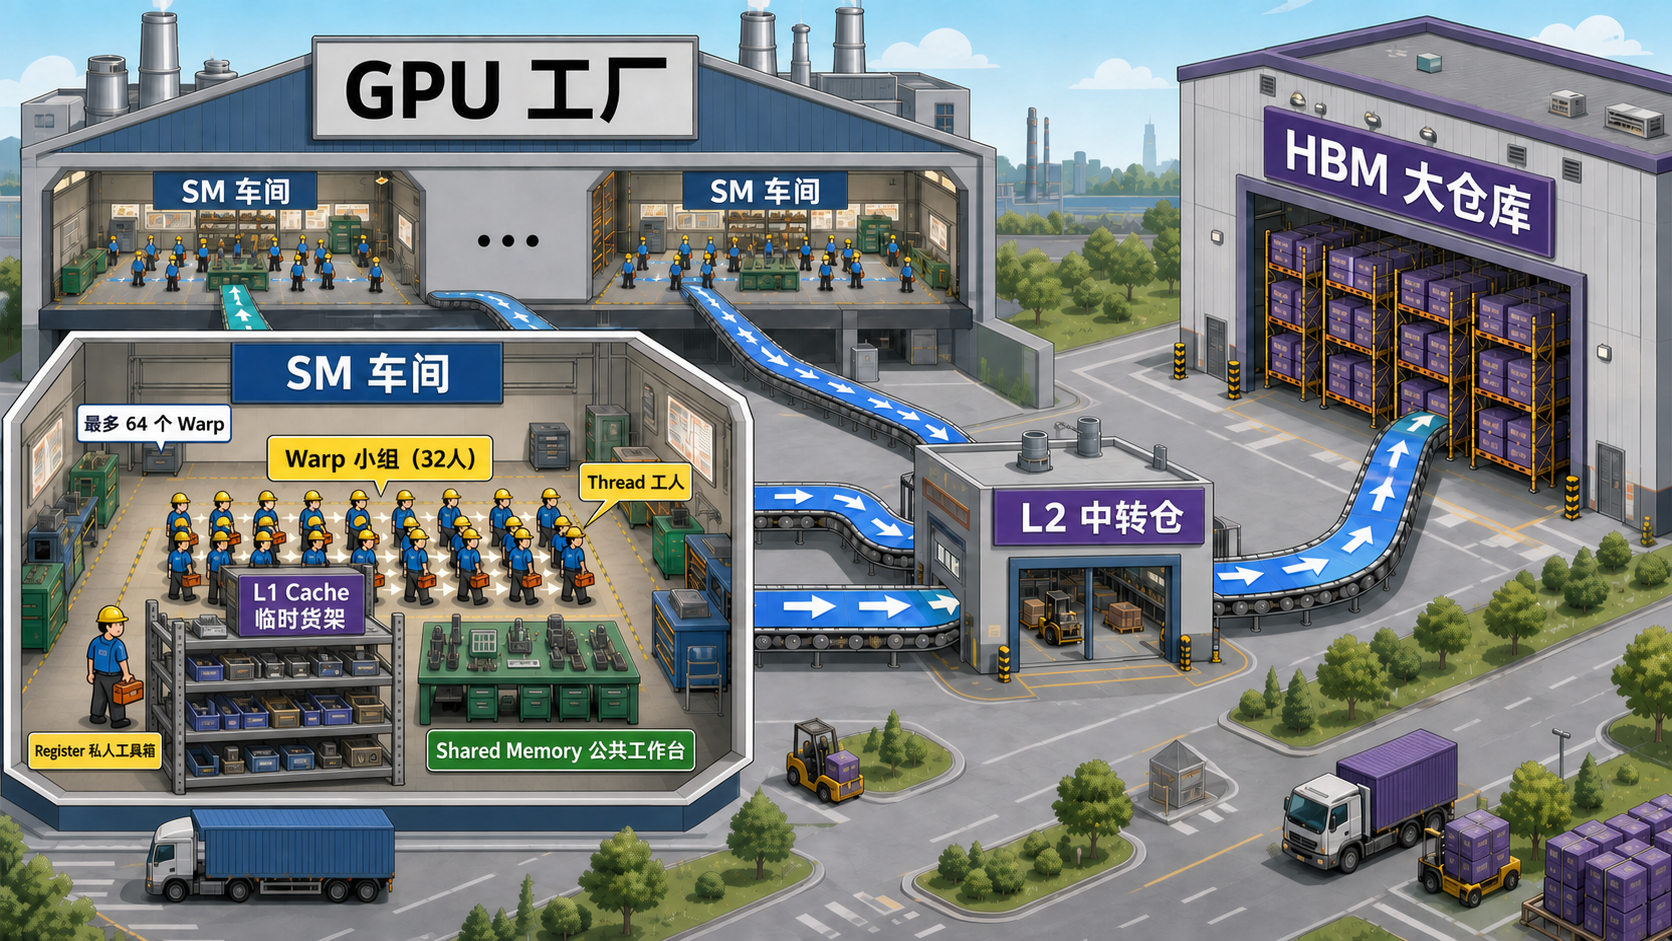
\includegraphics[height=0.78\textheight]{figs/analogy-gpu-factory.png}\\
  {\scriptsize SM = workshop \quad L2 = central depot \quad HBM = warehouse \quad (presenter's figure)}
\end{frame}
% ================================================================ 8
\begin{frame}{Four Warp Schedulers, Dual Issue}
  \begin{columns}[c]
    \column{0.58\textwidth}
    \begin{itemize}
      \item Each SM = four ``\kw{mini-SMs}'': independent warp schedulers with their own dispatch logic.
      \item Each scheduler issues \kw{1 warp instruction per cycle} $\Rightarrow$ up to
            \kw{4 warps advance per cycle}.
      \item \kw{Dual-issue}: one math (INT32/FP32/Tensor Core) \kw{+} one memory (load/store)
            instruction per cycle --- \emph{from the same warp}, never across warps.
      \item Best case: \kw{4 math + 4 memory} instructions in flight every cycle.
    \end{itemize}
    \column{0.38\textwidth}
    \centering
    {\small
    \begin{tabular}{@{}ll@{}}
      \toprule
      \textbf{Per cycle (Table 6-1)} & \textbf{Limit} \\
      \midrule
      Schedulers & 4 \\
      Warps issued & 4 \\
      Math / memory ops & 4 / 4 \\
      \bottomrule
    \end{tabular}}\\[6pt]
    {\scriptsize Book note: table values are illustrative;\\real benchmarks in the GitHub repo\refmark{7}}
  \end{columns}
  \pe{\kw{four dispatchers} on one floor, each sending out one crew per beat --- and a crew can compute with one hand while fetching parts with the other.}
\end{frame}

% ================================================================ 9
\begin{frame}{Analogy: One SM Is a Workshop}
  \begin{columns}[c]
    \column{0.54\textwidth}
    \centering
    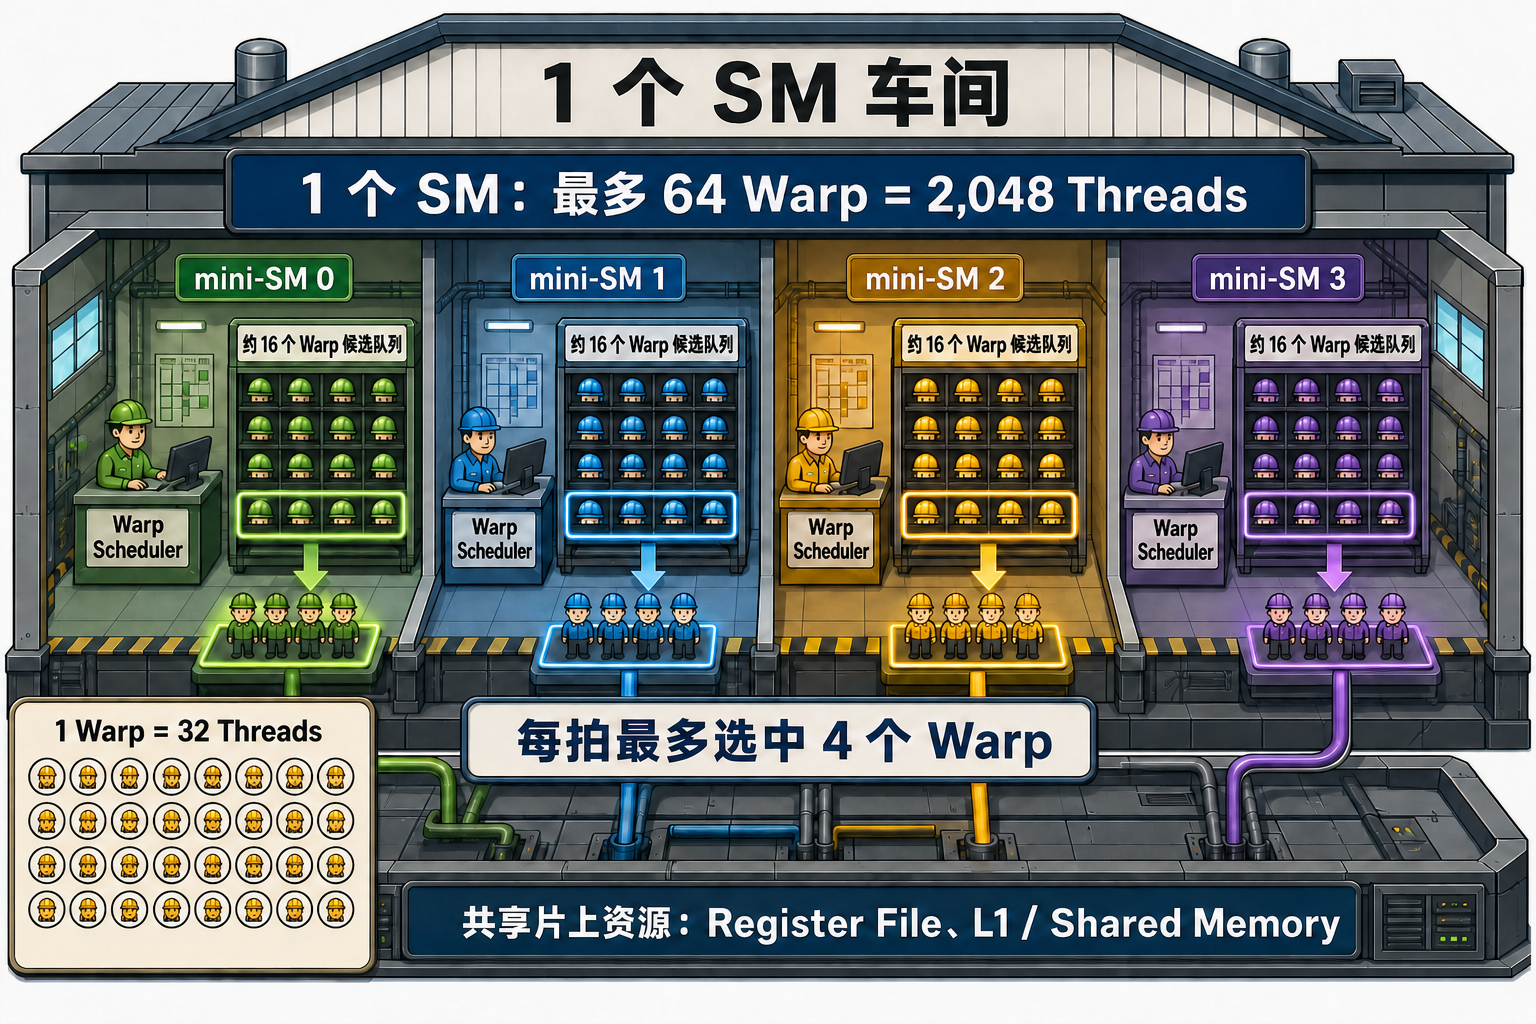
\includegraphics[width=0.86\linewidth]{figs/analogy-sm-workshop.png}\\
    {\scriptsize Presenter's analogy figure (not from the book)}
    \column{0.44\textwidth}
    \begin{itemize}\footnotesize
      \item Four bays = \kw{4 scheduling partitions} (``mini-SMs''), one
            \kw{warp scheduler} each --- CUDA only ever sees the whole SM.
      \item Hard hats on shelves = \kw{resident warps}: $\sim$16 per partition, \kw{64 total}.
            Resident = state already allocated --- \emph{not} ``executing right now.''
      \item Highlighted crews = the \kw{$\leq$4 warps issued this cycle}
            (each scheduler picks at most 1 \emph{ready} warp).
      \item Bottom left: \kw{1 warp = 32 threads} --- dispatched as a whole crew.
      \item Common foundation: \kw{register file, L1, shared memory} ---
            shared by all four partitions.
    \end{itemize}
  \end{columns}
  \pe{64 crews on standby, 4 dispatchers, at most 4 crews per beat --- each crew is 32 workers.}
\end{frame}

% ================================================================ 10
\begin{frame}{The Thread Hierarchy: Threads $\to$ Blocks $\to$ Grids}
  \begin{columns}[c]
    \column{0.52\textwidth}
    \begin{itemize}
      \item \kw{Thread}: runs your kernel code on one data element.
      \item \kw{Thread block} (CTA --- cooperative thread array): up to \kw{1{,}024 threads};
            shares fast on-chip \kw{shared memory}.
      \item \kw{Grid}: all blocks of one launch --- sized right, it scales to
            \kw{millions of threads} with zero kernel changes.
      \item The CUDA runtime (and PyTorch) handles scheduling and distribution across all SMs.
    \end{itemize}
    \column{0.45\textwidth}
    \centering
    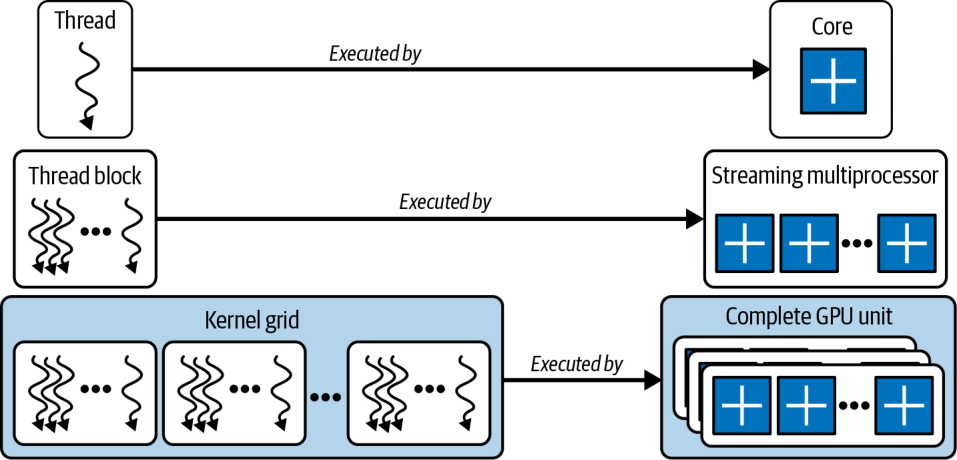
\includegraphics[width=\linewidth]{figs/fig6-3.png}\\
    {\scriptsize Figure 6-3. Threads, thread blocks (CTAs), and grids}
  \end{columns}
  \pe{workers (threads) form teams (blocks) that talk cheaply inside the team; the company (grid) hires as many teams as the job needs.}
\end{frame}

% ================================================================ 11
\begin{frame}{Blocks Cooperate Inside, Stay Independent Outside}
  \begin{columns}[c]
    \column{0.52\textwidth}
    \begin{itemize}
      \item Within a block: share data via shared memory, synchronize with
            \kw{\texttt{\_\_syncthreads()}} (a barrier: everyone arrives before anyone continues).
      \item \kw{Every barrier costs time} --- the book's advice: \kw{minimize synchronization points}.
      \item Across blocks: \kw{independent, no guaranteed order}. That freedom lets the scheduler
            spray blocks over all SMs --- and lets your kernel run \kw{unmodified on future GPUs}
            with more SMs.
    \end{itemize}
    \column{0.45\textwidth}
    \centering
    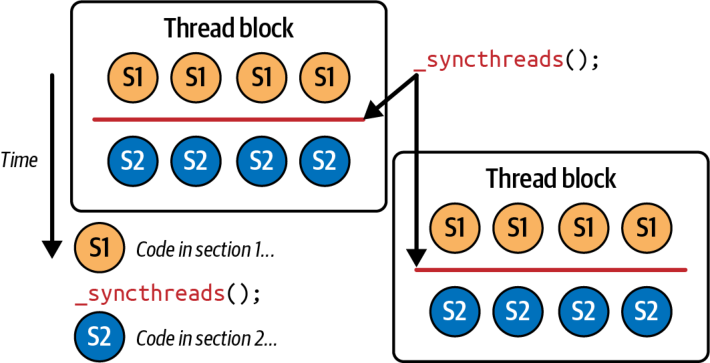
\includegraphics[width=0.9\linewidth]{figs/fig6-6.png}\\
    {\scriptsize Figure 6-6. \texttt{\_\_syncthreads()} between two code sections}
  \end{columns}
  \pe{team huddles (barriers) are useful but expensive --- call as few as possible; and never assume team A finishes before team B.}
\end{frame}

% ================================================================ 12
\begin{frame}{Thread Block Clusters and DSMEM}
  \bridge{* Good to know for LLM-scale matmuls --- not the focus of this session (details: Chapter 10).}
  \begin{columns}[c]
    \column{0.52\textwidth}
    \begin{itemize}\small
      \item Traditionally, threads in \emph{different} blocks could not cooperate. Modern GPUs add
            \kw{thread block clusters}: blocks that communicate \kw{across SMs},
            with cluster-scoped hardware barriers.
      \item Backed by \kw{DSMEM} (distributed shared memory): the shared-memory banks of
            participating SMs, linked over a fast \kw{on-chip interconnect} into one pool.
      \item Threads read, write, and atomically update each other's shared buffers
            \kw{at on-chip speeds --- without global-memory bandwidth}.
      \item Key enabler for huge matmuls in LLMs --- details in \kw{Chapter 10}.
    \end{itemize}
    \column{0.45\textwidth}
    \centering
    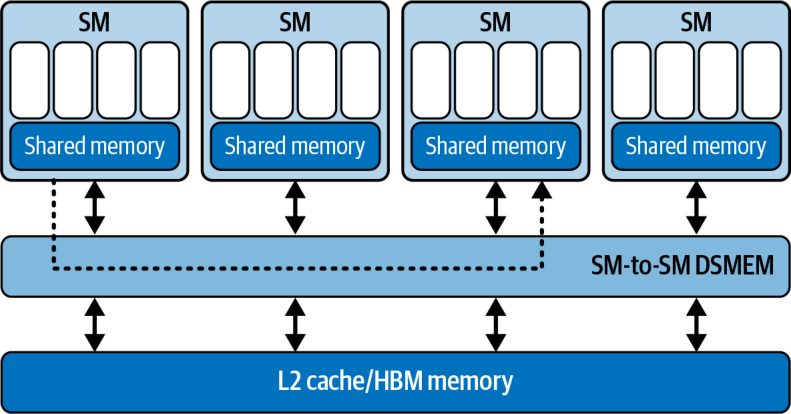
\includegraphics[width=\linewidth]{figs/fig6-5.png}\\
    {\scriptsize Figure 6-5. DSMEM shared across thread blocks in a cluster}
  \end{columns}
  \pe{neighboring teams knock a door through the wall between their workbenches instead of mailing parts through the warehouse.}
\end{frame}

% ================================================================ 13
\begin{frame}{Warps and SIMT: 32 Threads in Lockstep}
  \begin{columns}[c]
    \column{0.52\textwidth}
    \begin{itemize}
      \item Blocks are subdivided into \kw{warps of 32 threads} that execute one instruction
            together under \kw{SIMT} (single instruction, multiple threads).
      \item The warp --- not the thread --- is what the \kw{hardware actually schedules};
            warp size has been \kw{32 on every GPU generation}.
      \item The hardware hides long-latency events (global loads, cache fills, pipeline stalls)
            by \kw{rapidly switching among warps}.
    \end{itemize}
    \column{0.45\textwidth}
    \centering
    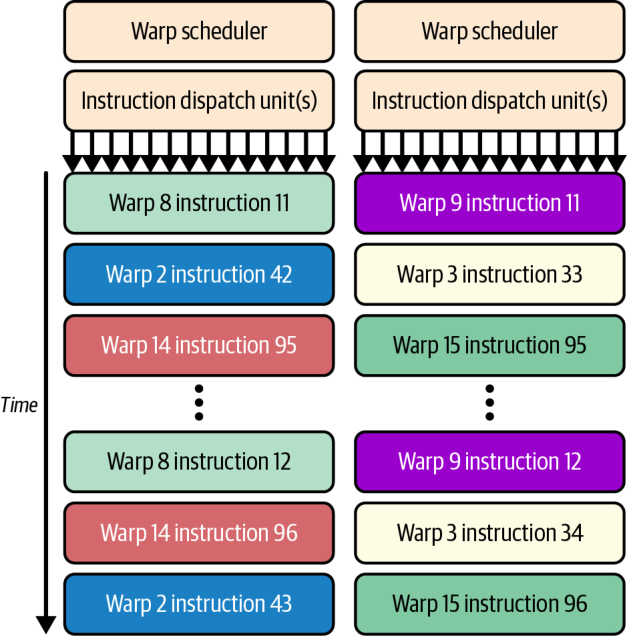
\includegraphics[width=0.8\linewidth]{figs/fig6-7.png}\\
    {\scriptsize Figure 6-7. A warp advances as a whole under the warp scheduler}
  \end{columns}
  \pe{a warp is a \kw{32-worker crew}: one instruction for all 32, everyone moves together --- or the whole crew waits.}
\end{frame}

% ================================================================ 14
\begin{frame}{Why SIMT Matters: One Instruction Drives 32 Lanes}
  \begin{columns}[c]
    \column{0.55\textwidth}
    \centering
    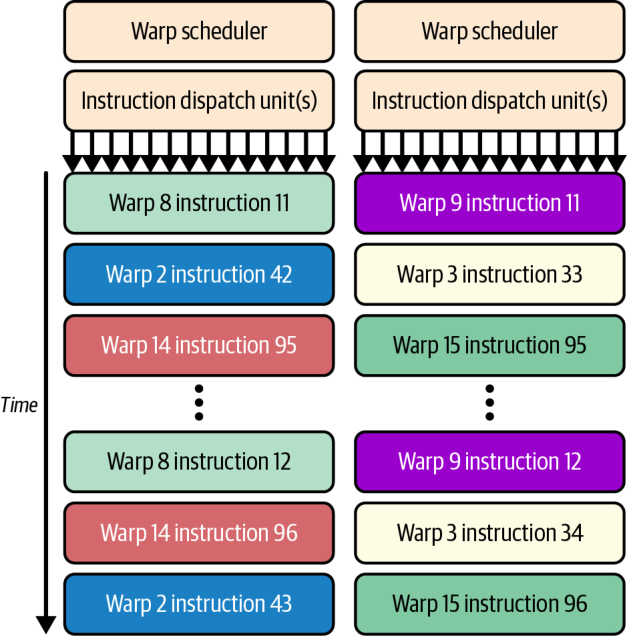
\includegraphics[width=0.66\linewidth]{figs/fig6-7.png}\\
    {\scriptsize Figure 6-7. The warp advances as a whole under the warp scheduler}
    \column{0.43\textwidth}
    \begin{itemize}\small
      \item The scheduler issues \kw{one instruction}; all \kw{32 lanes} execute it
            on \kw{32 different data elements}.
      \item Fetch / decode / schedule cost is paid \kw{once per warp}, not once per
            thread --- control logic shrinks, silicon goes to \kw{ALUs}.
      \item This is why the \kw{warp is the hardware's scheduling unit}:
            threads never advance alone; the crew moves together.
      \item The price of lockstep: if threads want \kw{different paths},
            the warp can't split --- next page.
    \end{itemize}
  \end{columns}
  \pe{one work order commands \kw{32 workers at once} --- cheap to manage, powerful when they agree, awkward when they don't.}
\end{frame}
% ================================================================ 15
\begin{frame}[fragile]{Warp Divergence: When \texttt{if/else} Splits the Crew}
  \begin{columns}[c]
    \column{0.52\textwidth}
\begin{lstlisting}
if (i % 2 == 0)
    taskA();   // 16 threads want this
else
    taskB();   // the other 16 want this
\end{lstlisting}
    \begin{itemize}\footnotesize
      \item A warp executes \kw{one instruction at a time} --- but here
            \kw{16 lanes want A} and \kw{16 want B}.
      \item So the warp runs \kw{A with the B-threads masked},
            then \kw{B with the A-threads masked} --- time $\approx$
            \kw{sum of both paths}.
      \item \kw{No penalty across warps} --- different warps branch freely.
      \item Fix: branch on \kw{warp-aligned} conditions (\texttt{i / 32}),
            not per-thread parity (\texttt{i \% 2}).
    \end{itemize}
    \column{0.44\textwidth}
    \centering
    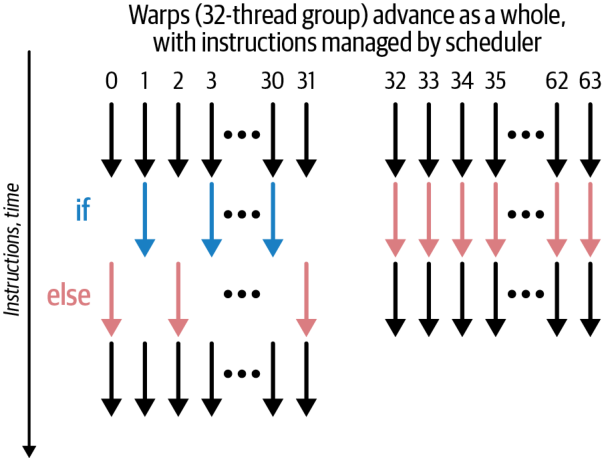
\includegraphics[width=0.8\linewidth]{figs/fig6-8.png}\\
    {\scriptsize Figure 6-8. Divergence (left) vs.\ uniform execution (right)}
  \end{columns}
  \pe{if half the \kw{crew} takes work order A and half takes B, the crew runs \kw{each job twice}.}
\end{frame}
% ================================================================ 16
\begin{frame}{Worked Example: One Million Adds Through Both Views}
  \begin{columns}[t]
    \column{0.46\textwidth}
    \begin{block}{Software view: you write the order sheet}
      \footnotesize
      \texttt{add<<<3907, 256>>>(A, B, C, N);}\\[4pt]
      {\scriptsize\setlength{\tabcolsep}{3pt}
      \begin{tabular}{@{}ll@{}}
        \toprule
        Grid & 1 (this launch) \\
        Blocks & \kw{3{,}907} $= \lceil 10^6/256 \rceil$ \\
        Threads / block & \kw{256} (your choice) \\
        Warps / block & \kw{8} (= 256 $\div$ 32, HW slices) \\
        Total & $\sim$1M threads, 31{,}256 warps \\
        \bottomrule
      \end{tabular}}\\[4pt]
      Each thread only says: ``I handle element \texttt{idx}.''
    \end{block}
    \column{0.50\textwidth}
    \begin{block}{Why 256 threads per block? (best practice)}
      \footnotesize
      \begin{itemize}
        \item \kw{Multiple of 32}: blocks are sliced into warps --- 256 = \kw{8 full warps},
              no half-empty warp wasting a scheduler slot.
        \item \kw{Well under the 1{,}024 cap}: each thread keeps enough \kw{registers},
              and the block's \kw{shared-memory} share stays modest.
        \item \kw{Small enough to stack}: an SM hosts \kw{several 256-thread blocks} at once
              $\Rightarrow$ many resident warps $\Rightarrow$ \kw{latency hiding}.
        \item Not magic: \kw{128--512} are all reasonable --- \kw{profile} to pick.
      \end{itemize}
    \end{block}
  \end{columns}
  \smallskip
  \begin{itemize}\footnotesize
    \item 4 SMs or 400 SMs: \kw{same code} --- the grid \kw{decouples} the program from the GPU's size.
  \end{itemize}
  \pe{you write the \kw{order sheet} (3,907 teams of 256 workers); the hardware assigns teams to workshops and slices each team into 32-worker crews.}
\end{frame}

% ================================================================ 17
\begin{frame}{Let the Workshop Move: Latency Hiding, Cycle by Cycle}
  \begin{columns}[t]
    \column{0.48\textwidth}
    \begin{block}{One partition, one moment}
      \small
      Warp A --- \kw{waiting} on an HBM load\\
      Warp B --- \kw{waiting} on a previous result\\
      Warp C --- \kw{ready}\qquad Warp D --- \kw{ready}\\[4pt]
      The scheduler skips A and B and \kw{issues C or D} ---
      skipping a stalled warp costs \kw{nothing}.
    \end{block}
    {\small
    \begin{tabular}{@{}ll@{}}
      \toprule
      \textbf{Cycle} & \textbf{Issued (example)} \\
      \midrule
      1 & Warp C \\
      2 & Warp F \\
      3 & Warp D \\
      4 & Warp H \\
      \bottomrule
    \end{tabular}}
    \column{0.48\textwidth}
    \begin{itemize}
      \item ``Issued'' = the instruction \kw{starts}; it need not finish this cycle.
      \item Latency hiding does \kw{not} shorten any warp's wait ---
            it \kw{fills the wait} with other warps' work.
      \item This is why \kw{64 resident warps} matter: a deep pool of \emph{ready}
            candidates for the 4 dispatchers --- and why low occupancy hurts
            (nothing ready to switch to).
    \end{itemize}
  \end{columns}
  \pe{latency hiding does \kw{not} reduce waiting time --- it \kw{fills the waiting time} with other crews' work.}
\end{frame}

% ================================================================ 18
\begin{frame}{Occupancy Gives the Scheduler More Choices}
  \begin{block}{Definition}
    \kw{Occupancy} = active warps on an SM $\div$ the hardware maximum (64 on Blackwell).
    ``\kw{Achieved occupancy}'' is the measured average, reported by Nsight Compute.
  \end{block}
  \begin{columns}[t]
    \column{0.48\textwidth}
    \begin{itemize}
      \item High occupancy $\Rightarrow$ when one warp stalls on memory, another is ready
            $\Rightarrow$ \kw{latency hiding}.
      \item Blackwell's large register file (64K/SM) makes high occupancy easier to reach.
    \end{itemize}
    \column{0.48\textwidth}
    \begin{itemize}
      \item The counterweight: warps share \kw{registers and shared memory}. Pack in too many
            $\Rightarrow$ \kw{register spilling} to slow memory --- a new stall you created.
      \item So: profile occupancy \kw{together with} register / shared-memory usage.
    \end{itemize}
  \end{columns}
  \pe{occupancy is \kw{not} ``how busy the GPU is'' and \kw{not} a performance score --- it counts \kw{how many resident crews the dispatcher can choose from}. Enough hides latency; beyond enough, more may not help (p.~52).}
\end{frame}

% ================================================================ 19
\begin{frame}{Hardware Limits I: Warp and Block (Table 6-2)}
  \bridge{No need to memorize these numbers. The one idea: each block's threads, registers, and shared memory decide how many blocks and warps still fit on one SM.}
  \begin{columns}[c]
    \column{0.52\textwidth}
    {\small
    \begin{tabular}{@{}ll@{}}
      \toprule
      \textbf{Resource} & \textbf{Limit (B200)} \\
      \midrule
      Warp size & 32 threads \\
      Max threads / block & 1{,}024 \\
      Max warps / block & 32 \ (= 1024 $\div$ 32) \\
      \bottomrule
    \end{tabular}}\\[6pt]
    {\scriptsize \texttt{blockDim.x $\times$ blockDim.y $\times$ blockDim.z $\leq$ 1024}}
    \column{0.45\textwidth}
    \begin{block}{Why multiples of 32 matter}
      \small A \kw{33-thread block} occupies \kw{two} warp slots --- the second warp runs
      \kw{1 of 32 lanes} but still consumes a full scheduler slot. Every non-multiple of 32
      donates scheduler capacity to the void.
    \end{block}
  \end{columns}
  \medskip
  \begin{itemize}
    \item Block too big $\Rightarrow$ too many registers per block $\Rightarrow$ \kw{spilling};
          or too much shared memory (227 KB usable is shared by \kw{all resident blocks} on the SM).
    \item Smaller blocks can mean \kw{higher occupancy} --- more independent blocks fit per SM.
  \end{itemize}
\end{frame}

% ================================================================ 20
\begin{frame}{Hardware Limits II: SM-Resident and Grid (Tables 6-3 / 6-4)}
  \begin{columns}[c]
    \column{0.55\textwidth}
    {\small\setlength{\tabcolsep}{4pt}
    \begin{tabular}{@{}ll@{}}
      \toprule
      \textbf{Per SM (resident)} & \textbf{Limit} \\
      \midrule
      Max warps & \kw{64} (= 2{,}048 threads) \\
      Max threads & 2{,}048 \\
      Max blocks & 32 \\
      \midrule
      \textbf{Grid} & \\
      \midrule
      Max blocks (X / Y / Z) & $\sim$2.1B / 65{,}535 / 65{,}535 \\
      Max concurrent grids & \kw{128} kernels per device \\
      \bottomrule
    \end{tabular}}
    \column{0.42\textwidth}
    \centering
    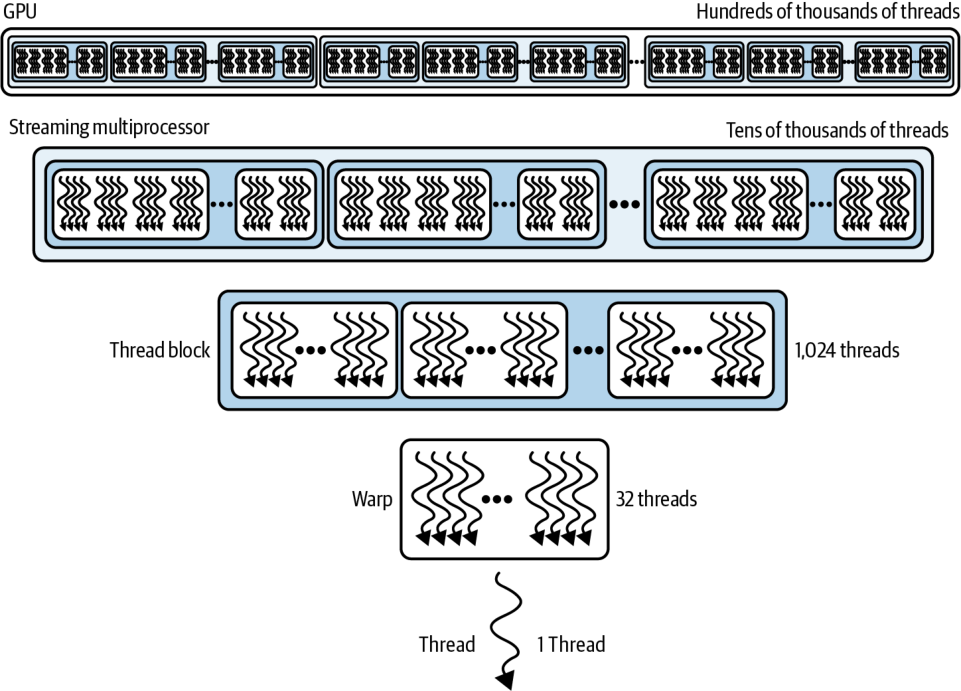
\includegraphics[width=\linewidth]{figs/fig6-9.png}\\
    {\scriptsize Figure 6-9. Relative scale of thread resources}
  \end{columns}
  \medskip
  \begin{itemize}\small
    \item Worked example: 1024-thread blocks $\Rightarrow$ only \kw{2 blocks/SM};
          256-thread blocks $\Rightarrow$ \kw{8 blocks/SM} --- same 2{,}048 threads, more flexibility.
    \item In practice you hit \kw{per-SM limits} long before grid limits;
          $>$65{,}535 blocks in Y/Z $\Rightarrow$ use 2D/3D grids or multilaunch.\refmark{1,2}
  \end{itemize}
\end{frame}

% ================================================================ 21
\begin{frame}{Compatibility: PTX, SASS, and Fatbins}
  \begin{columns}[t]
    \column{0.48\textwidth}
    \begin{itemize}
      \item \kw{SASS}: final machine code for \emph{one} architecture (sm\_90 = Hopper,
            sm\_100 = Blackwell). SASS-only binaries \kw{won't run on newer GPUs}.
      \item \kw{PTX}: virtual ISA the driver \kw{JIT-compiles} at load time $\Rightarrow$
            \kw{forward compatibility}.
      \item Family targets (\texttt{sm\_100f}) restrict portability to the same feature family.
    \end{itemize}
    \column{0.48\textwidth}
    \begin{block}{Best practice}
      \small Ship a \kw{fatbin}: generic PTX \kw{+} the family-specific cubins you need for
      optimizations --- with \kw{fallback paths} for other architectures.
    \end{block}
    \begin{itemize}\small
      \item Verify with \kw{\texttt{CUDA\_FORCE\_PTX\_JIT=1}}: forces PTX JIT;
            if the binary lacks PTX, \kw{kernel launch fails} --- rebuild with PTX.
    \end{itemize}
  \end{columns}
  \pe{fast code must also \kw{survive GPU generations} --- ship optimized \kw{SASS} for today's chips plus \kw{PTX} for forward compatibility.}
\end{frame}


\end{document}
